\begin{figure}
	\begin{center}
		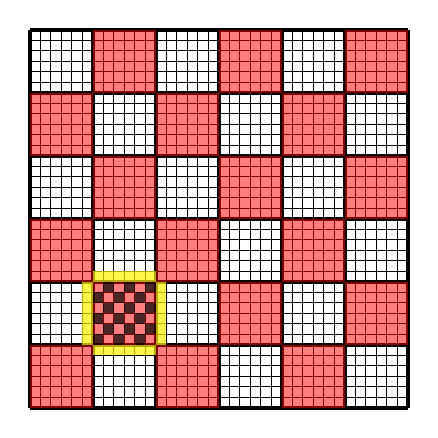
\begin{tikzpicture}[x=0.8cm,y=0.8cm]
		
		\foreach \p in {0,1,...,6}{
				\draw [ultra thick] (\p,0) -- (\p,6);
				\draw [ultra thick] (0,\p) -- (6,\p);
			}
		\foreach \p in {0,0.5,...,18}{
				\draw (\p/3,0) -- (\p/3,6);
				\draw (0,\p/3) -- (6,\p/3);
			}

		\foreach \blockx in {0,2,...,5}{
				\foreach \blocky in {0,2,...,5}{
					\fill [fill=red, opacity=0.5] (\blockx,\blocky) rectangle (\blockx+1,\blocky+1);
			}
		}
		\foreach \blockx in {0,2,...,5}{
				\foreach \blocky in {0,2,...,5}{
					\fill [fill=red, opacity=0.5] (\blockx+1,\blocky+1) rectangle (\blockx+2,\blocky+2);
			}
		}

		\fill [fill=yellow, opacity=0.7] (1,2) rectangle (2,2+0.5/3);
		\fill [fill=yellow, opacity=0.7] (1,1) rectangle (1-0.5/3,2);
		\fill [fill=yellow, opacity=0.7] (1,1) rectangle (2,1-0.5/3);
		\fill [fill=yellow, opacity=0.7] (2,1) rectangle (2+0.5/3,2);

		\foreach \a in {0,2,...,5}{
				\foreach \b in {0,2,...,5}{
					\fill [fill=black, opacity=0.7] (1+\a*0.5/3,1+\b*0.5/3) rectangle (1+\a*0.5/3+0.5/3,1+\b*0.5/3+0.5/3);
			}
	}
		\foreach \a in {0,2,...,5}{
				\foreach \b in {0,2,...,5}{
					\fill [fill=black, opacity=0.7] (1+\a*0.5/3+0.5/3,1+\b*0.5/3+0.5/3) rectangle (1+\a*0.5/3+2*0.5/3,1+\b*0.5/3+2*0.5/3);
			}
	}

		\end{tikzpicture}
	\end{center}
	\caption{Le zone rosse pi\`u le aree gialle rappresentano i blocchi di memoria \emph{shared}. Ogni blocco viene aggiornato a scacchiera. Le condizioni di raccordo blocco-blocco sono identificate dai siti reticolari colorati in giallo}
	\label{reticolo_shared}
\end{figure}

